\section*{Esercizi del 2 maggio}

\subsection*{Esercizio 4.2}
Siano $K\subs S^3$ un nodo, $\nu K$ un intorno tubolare (aperto) di $K$ tale che $\overline{\nu K}$ sia diffeomorfo a $D^2\times S^1$. Allora $M=S^3\setminus\nu K$ è una $3$-varietà compatta il cui bordo $\del M=\overline{\nu K}\setminus \nu K$ è diffeomorfo al $2$-toro $T^2$. Per semplicità, poniamo $T^2=\del M$ e $D^2\times S^2=\nu K$.

Scriviamo una parte della successione esatta di Mayer-Vietoris\footnote{Nonostante $M$ e $D^2\times S^1$ non siano aperti in $S^3$, entrambi sono retratti per deformazione di un loro intorno aperto; inoltre tali intorni aperti si possono scegliere in modo che la loro intersezione si retragga per deformazione su $M\cap (D^2\times S^1)=T^2$.} per $S^3=M\cup (D^2\times S^1)$, dove $\map{i}{T^2}{M}$ e $\map{j}{T^2}{D^2\times S^1}$ indicano le inclusioni:
\begin{diagram}[column sep=large]
H_2(S^3)\rar&H_1(T^2)\rar["{(i_*,j_*)}"]&H_1(M)\dirsum H_1(D^2\times S^1)\rar&H_1(S^3).
\end{diagram}
Ricordando che $H_2(S^3)=H_1(S^3)=0$ otteniamo l'isomorfismo
\begin{diagram}[column sep=large]
0\rar&H_1(T^2)\rar["{(i_*,j_*)}","\iso"']&H_1(M)\dirsum H_1(D^2\times S^1)\rar&0.
\end{diagram}
Poiché $H_1(T^2)=\ZZ\dirsum\ZZ$ e $H_1(D^2\times S^1)=\ZZ$, otteniamo immediatamente che $H_1(M)=\ZZ$.

Sia ora $l\in H_1(T^2)$ la classe di omologia, ben definita a meno del segno, tale che $i_*(l)=0\in H_1(M)$ e $j_*(l)$ generi $H_1(D^2\times S^1)$. Osserviamo che il nucleo dell'omomorfismo $\map{i_*}{H_1(T^2)}{H_1(M)}$ è precisamente il sottogruppo ciclico generato da $l$, e che $l$ è primitivo, in quanto $H_1(M)=\ZZ$ non ha torsione. Sappiamo allora che esiste un'unica classe di isotopia di curve semplici chiuse non orientate che rappresenta $l$ in omologia; poiché anche $-l$ è rappresentata dalla stessa classe di isotopia, otteniamo che è ben definita la \defterm{longitudine} come l'unica curva semplice chiusa di $T^2$ (a meno di isotopia e dell'orientazione) che in omologia genera il nucleo di $i_*$.

Con un ragionamento del tutto analogo, possiamo ben definire il \defterm{meridiano} come l'unica curva semplice chiusa di $T^2$ (a meno di isotopia e dell'orientazione) che in omologia genera il nucleo dell'omomorfismo $\map{j_*}{H_1(T^2)}{H_1(D^2\times S^1)}$.


\newpage
\subsection*{Esercizio 4.3}
\tikzfading[name=fade out,inner color=transparent!0,outer color=transparent!100]
\tikzset{
pics/tetrahedron/.style={
code={
\coordinate (#1-1) at (0,0);
\coordinate (#1-2) at (1.8,-.7);
\coordinate (#1-3) at (2.5,.4);
\coordinate (#1-4) at (1,1.8);
}},
on each segment/.style={
decorate,
decoration={
show path construction,
lineto code={\path [#1] (\tikzinputsegmentfirst) -- (\tikzinputsegmentlast);},
closepath code={\path [#1] (\tikzinputsegmentfirst) -- (\tikzinputsegmentlast);}
}},
mid arrow/.style={postaction={decorate,decoration={
markings,
mark=at position .5 with {\arrow[scale=1.5,#1]{latex}}
}}},
}
Ricordiamo che una struttura iperbolica sul complementare del nodo figura otto è data dall'incollamento di due tetraedri ideali regolari iperbolici secondo il seguente schema (le facce dello stesso colore vengono identificate, in modo da rispettare le frecce e i colori rappresentati sugli spigoli).

\begin{center}
\begin{tikzpicture}
\pic[scale=1.5] at (0,0) {tetrahedron=a};
\pic[scale=1.5] at (6,0) {tetrahedron=b};
\foreach \T in {a,b} {
\begin{scope}[on background layer={opacity=.4}]
\fill[orange] (\T-1) -- (\T-2) -- (\T-3) -- cycle;
\fill[green] (\T-1) -- (\T-3) -- (\T-4) -- cycle;
\end{scope}
\begin{scope}[opacity=.3]
\fill[white] (\T-1) -- (\T-2) -- (\T-4) -- cycle;
\fill[black] (\T-2) -- (\T-3) -- (\T-4) -- cycle;
\end{scope}
}
\draw[blue,thick,postaction={on each segment={mid arrow}}] (a-1) -- (a-2) (a-3) -- (a-2) (a-3) -- (a-4) (b-2) -- (b-3) (b-2) -- (b-4);
\draw[red,thick,postaction={on each segment={mid arrow}}] (a-1) -- (a-4) (a-2) -- (a-4) (b-2) -- (b-1) (b-4) -- (b-1) (b-4) -- (b-3);
\begin{scope}[on background layer={thick,opacity=.7,dashed}]
\draw[blue,postaction={mid arrow}] (b-1) -- (b-3);
\draw[red,postaction={mid arrow}] (a-1) -- (a-3);
\end{scope}
\foreach \T in {a,b} {
\foreach \i/\pos in {1/east,2/north,3/west,4/south} {
\draw[fill=white] (\T-\i) circle (2pt);
\node[inner sep=5pt,anchor=\pos] at (\T-\i) {$\T_{\i}$};
}}
\node[anchor=east] at ($(a-4)+(-1.5,-.5)$) {$T\times\{0\}$};
\node[anchor=west] at ($(b-4)+(2,-.5)$) {$T\times\{1\}$};
\end{tikzpicture}
\end{center}

Per fissare la notazione, siano $M$ il complementare del nodo figura otto, $T\times\{0,1\}$ l'unione disgiunta dei due tetraedri $T\times\{0\}$ e $T\times\{1\}$, $\sim$ la relazione di equivalenza descritta dall'incollamento, in modo che $M=T\times\{0,1\}/\sim$. Ricordiamo che, essendo $T$ un tetraedro ideale regolare iperbolico, ogni permutazione dei suoi vertici è indotta da un'isometria di $\HH^3$. Sia allora $\map{g}{T}{T}$ l'isometria di $T$ che induce la permutazione $\sigma=(1\;2)(3\;4)$.
\begin{center}
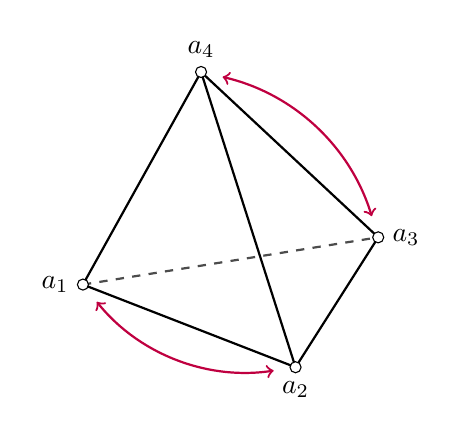
\begin{tikzpicture}
\pic[scale=1.5] {tetrahedron=a};
\draw[thick,opacity=.7,dashed] (a-1) -- (a-3);
\draw[thick,line join=bevel] (a-2) -- (a-1) -- (a-4) -- (a-2) -- (a-3) -- (a-4);
\begin{scope}[thick,purple,<->,shorten <=8pt,shorten >=8pt]
\draw (a-1) to[bend right] (a-2);
\draw (a-3) to[bend right] (a-4);
\end{scope}
\foreach \i/\pos in {1/east,2/north,3/west,4/south} {
\draw[fill=white] (a-\i) circle (2pt);
\node[inner sep=5pt,anchor=\pos] at (a-\i) {$a_\i$};
}
\end{tikzpicture}
\end{center}
Definiamo l'isometria
\Map{f}{T\times\{0,1\}}{T\times\{0,1\}}{(x,i)}{(g(x),1-i).}
In altre parole, $f$ scambia $T\times\{0\}$ e $T\times\{1\}$, e poi applica a ognuno dei tetraedri l'isometria che induce la permutazione $\sigma$. In altre parole ancora, $f$ è l'unica isometria di $T\times\{0,1\}$ che effettua i seguenti scambi di vertici:
\begin{align*}
a_1\leftrightarrow b_2&&a_2\leftrightarrow b_1&&a_3\leftrightarrow b_4&&a_4\leftrightarrow b_3.
\end{align*}
È facile verificare che $f$ è compatibile con la relazione di equivalenza $\sim$.
\begin{itemize}
\item Per quanto riguarda le facce, consideriamo ad esempio $a_1a_2a_3$ e $b_2b_3b_1$, identificate da $\sim$. La faccia $a_1a_2a_3$ viene mandata da $f$ in $b_2b_1b_4$, mentre $b_2b_3b_1$ viene mandata in $a_1a_4a_2$; le facce $a_1a_4a_2$ e $b_2b_1b_4$ risultano identificate da $\sim$. Analogamente si mostra che $f$ è compatibile con $\sim$ sulle parti interne di tutte le altre facce.
\item Per quanto riguarda gli spigoli, una verifica diretta mostra che $f$ manda spigoli rossi in spigoli blu e viceversa, preservando la direzione delle frecce. Pertanto $f$ risulta compatibile con $\sim$ anche sugli spigoli.
\end{itemize}
Per passaggio al quoziente otteniamo dunque un'isometria $\map{\overline{f}}{M}{M}$. Verifichiamo che $\overline{f}$ non ha punti fissi.
\begin{itemize}
\item I punti delle parti interne dei tetraedri non sono fissati da $\overline{f}$, poiché $f$ scambia $T\times\{0\}$ e $T\times\{1\}$.
\item I punti delle parti interne delle facce non sono fissati da $\overline{f}$, poiché $g$ agisce in modo libero sull'insieme delle facce di $T$.
\item I punti degli spigoli non sono fissati da $\overline{f}$, poiché (come già osservato) $f$ manda spigoli rossi in spigoli blu e viceversa.
\end{itemize}

Osserviamo infine che $\overline{f}$ ha ordine 2. Pertanto possiamo definire $N=M/\langle\overline{f}\rangle$, che risulta essere una varietà iperbolica di volume finito, doppiamente rivestita dal complementare del nodo figura otto. La proiezione al quoziente della tassellazione di $M$ fornisce una tassellazione di $N$ con un tetraedro ideale regolare iperbolico, che riportiamo per completezza.
\begin{center}
\begin{tikzpicture}
\pic[scale=1.5] {tetrahedron=a};
\begin{scope}[on background layer={opacity=.4}]
\fill[orange] (a-1) -- (a-2) -- (a-3) -- cycle;
\fill[blue!20] (a-1) -- (a-3) -- (a-4) -- cycle;
\end{scope}
\begin{scope}[opacity=.4]
\fill[orange] (a-1) -- (a-2) -- (a-4) -- cycle;
\fill[blue!20] (a-2) -- (a-3) -- (a-4) -- cycle;
\end{scope}
\scoped[on background layer]\draw[thick,dashed, opacity=.7] (a-1) -- (a-3);
\draw[thick] (a-1) -- (a-2) (a-1) -- (a-4) (a-2) -- (a-4) (a-3) -- (a-2) (a-3) -- (a-4);
\foreach \i/\pos in {1/east,2/north,3/west,4/south} {
\draw[fill=white] (a-\i) circle (2pt);
\node[inner sep=5pt,anchor=\pos] at (a-\i) {$a_{\i}$};
}
\end{tikzpicture}
\end{center}
La varietà $N$ si ottiene incollando la faccia $a_1a_2a_3$ su $a_1a_4a_2$ e la faccia $a_1a_3a_4$ su $a_3a_2a_4$.

\newpage
\subsection*{Esercizio 4.4}
\tikzset{
pics/octahedron/.style={
code={
\coordinate (#1-1) at (0,1,0);
\coordinate (#1-2) at (1,0,0);
\coordinate (#1-3) at (0,0,1);
\coordinate (#1-4) at (-1,0,0);
\coordinate (#1-5) at (0,0,-1);
\coordinate (#1-6) at (0,-1,0);
}}}
Ricordiamo la costruzione, vista a lezione, di una $3$-varietà iperbolica tassellata da quattro ottaedri ideali regolari iperbolici. Dopo aver colorato le facce degli ottaedri a scacchiera, le identifichiamo secondo il seguente schema, utilizzando come mappa di incollamento l'identità.

\begin{center}
\begin{tikzpicture}[z={(6pt,8pt)},every pic/.style={scale=1.2}]
\pic at (0,0) {octahedron={o1}};
\pic at (6,0) {octahedron={o2}};
\pic at (0,-4.5) {octahedron={o3}};
\pic at (6,-4.5) {octahedron={o4}};
\foreach \w in {o1,o2,o3,o4} {
    \fill[opacity=.4,white] (\w-1) -- (\w-2) -- (\w-3) -- cycle (\w-3) -- (\w-4) -- (\w-6) -- cycle;
    \fill[opacity=.4,orange] (\w-1) -- (\w-3) -- (\w-4) -- cycle (\w-2) -- (\w-3) -- (\w-6) -- cycle;
    \draw[dashed,opacity=.7,line join=round] (\w-1) -- (\w-3) -- (\w-6) (\w-2) -- (\w-3) -- (\w-4);
    \draw[fill=white] (\w-3) circle (2pt);
    \fill[opacity=.4,white] (\w-2) -- (\w-5) -- (\w-6) -- cycle (\w-1) -- (\w-4) -- (\w-5) -- cycle;
    \fill[opacity=.4,orange] (\w-4) -- (\w-5) -- (\w-6) -- cycle (\w-1) -- (\w-2) -- (\w-5) -- cycle;
    \draw[line join=round] (\w-1) -- (\w-2) -- (\w-6) -- (\w-4) -- (\w-1) -- (\w-5) -- (\w-6) (\w-2) -- (\w-5) -- (\w-4);
    \foreach \i in {1,2,4,5,6} {
        \draw[fill=white] (\w-\i) circle (2pt);
    }
}
\begin{scope}[thick,double distance=3pt,{Implies}-{Implies},line cap=round,shorten <=10pt,shorten >=10pt]
\draw[double=orange!40] (o1-2) -- (o2-4);
\draw[double=orange!40] (o3-2) -- (o4-4);
\draw[double=white] (o1-6) -- (o3-1);
\draw[double=white] (o2-6) -- (o4-1);
\end{scope}
\node[anchor=east] at ($(o1-4)+(-.5,.5)$) {$O\times\{0\}$};
\node[anchor=west] at ($(o2-2)+(.5,.5)$) {$O\times\{1\}$};
\node[anchor=east] at ($(o3-4)+(-.5,.5)$) {$O\times\{2\}$};
\node[anchor=west] at ($(o4-2)+(.5,.5)$) {$O\times\{3\}$};
\end{tikzpicture}
\end{center}

Seguiamo ora un approccio simile a quello dell'esercizio precedente. Siano $O\times\{0\}$, $O\times\{1\}$, $O\times\{2\}$, $O\times\{3\}$ gli ottaedri, $M=O\times\{0,1,2,3\}/\sim$ la varietà ottenuta mediante l'incollamento. Sia $\map{g}{O}{O}$ l'isometria data dalla rotazione di un angolo piatto attorno alla retta che congiunge due vertici diametralmente opposti.
\begin{center}
\begin{tikzpicture}[z={(6pt,8pt)}]
\pic[scale=1.8] {octahedron=a};
\begin{scope}[thick,line join=round]
\draw[dashed,opacity=.7] (a-1) -- (a-3) -- (a-6) (a-2) -- (a-3) -- (a-4);
\draw[purple,dashed] (a-1) -- (a-6);
\draw[line join=round] (a-1) -- (a-2) -- (a-6) -- (a-4) -- (a-1) -- (a-5) -- (a-6) (a-2) -- (a-5) -- (a-4);
\draw[-{Latex[slant=0]},purple] (0,0,-.5) to[out=0,in=0,looseness=5] (0,0,.5);
\end{scope}
\foreach \i in {1,...,6} {\draw[fill=white] (a-\i) circle (2pt);}
\end{tikzpicture}
\end{center}
Definiamo l'isometria
\Map{f}{O\times\{0,1,2,3\}}{O\times\{0,1,2,3\}}{(x,i)}{(g(x),3-i).}
In altre parole, $f$ scambia $(O\times\{0\})\leftrightarrow (O\times\{3\})$ e $(O\times\{1\})\leftrightarrow (O\times\{2\})$, e poi applica $g$ a ciascun ottaedro. Si vede facilmente che $f$ è compatibile con la relazione di equivalenza $\sim$, grazie al fatto che $g$ preserva la colorazione a scacchiera (la compatibilità sugli spigoli si può verificare direttamente a parte). Per passaggio al quoziente otteniamo dunque un'isometria $\map{\overline{f}}{M}{M}$. Si vede immediatamente che $\overline{f}$ agisce su $M$ senza punti fissi. Infatti tutte le identificazioni in $O\times\{0,1,2,3\}$ sono del tipo $(x,i)\sim(x,i')$; se $(x,i)$ è tale che $f(x,i)\sim (x,i)$, allora necessariamente $g(x)=x$, dunque $x$  è un punto fisso per $g$ e di conseguenza appartiene alla parte interna di $O$. Poiché i punti nelle parti interne degli ottaedri non sono identificati con altri punti, dovrebbe valere che $3-i=i$, il che è assurdo.

Osserviamo infine che $\overline{f}$ ha ordine $2$. Pertanto possiamo definire $N=M/\langle\overline{f}\rangle$, che risulta essere una varietà iperbolica di volume finito, doppiamente rivestita da $M$. La proiezione al quoziente della tassellazione di $M$ fornisce una tassellazione di $N$ con due ottaedri ideali regolari iperbolici, che riportiamo per completezza.

\begin{center}
\begin{tikzpicture}[z={(6pt,8pt)}]
\pic[scale=1.8] {octahedron=a};
\pic[scale=1.8] at (6,0) {octahedron=b};
\foreach \w in {a,b} {
    \fill[opacity=.4,white] (\w-1) -- (\w-2) -- (\w-3) -- cycle (\w-3) -- (\w-4) -- (\w-6) -- cycle;
    \fill[opacity=.4,green!70!blue] (\w-1) -- (\w-3) -- (\w-4) -- cycle (\w-2) -- (\w-3) -- (\w-6) -- cycle;
    \draw[dashed,opacity=.7,line join=round] (\w-1) -- (\w-3) -- (\w-6) (\w-2) -- (\w-3) -- (\w-4);
    \draw[fill=white] (\w-3) circle (2pt);
    \node[inner sep=5pt,anchor=north west] at (\w-3) {$\w_3$};
    \fill[opacity=.4,white] (\w-2) -- (\w-5) -- (\w-6) -- cycle (\w-1) -- (\w-4) -- (\w-5) -- cycle;
    \fill[opacity=.4,green!70!blue] (\w-4) -- (\w-5) -- (\w-6) -- cycle (\w-1) -- (\w-2) -- (\w-5) -- cycle;
    \draw[line join=round] (\w-1) -- (\w-2) -- (\w-6) -- (\w-4) -- (\w-1) -- (\w-5) -- (\w-6) (\w-2) -- (\w-5) -- (\w-4);
    \foreach \i/\pos in {1/south,2/north west,4/north east,5/north west,6/north} {
        \draw[fill=white] (\w-\i) circle (2pt);
        \node[inner sep=5pt,anchor=\pos] at (\w-\i) {$\w_{\i}$};
    }
}
\end{tikzpicture}
\end{center}

Ogni faccia azzurra a sinistra si identifica con la corrispondente faccia azzurra a destra, usando l'identità come mappa di incollamento. Le facce bianche si identificano invece mediante il seguente schema:
\begin{align*}
a_1a_2a_3\leftrightarrow b_1b_4b_5&&a_1a_4a_5\leftrightarrow b_1b_2b_3&&a_6a_3a_4\leftrightarrow b_6b_5b_2&&a_6a_5a_2\leftrightarrow b_6b_3b_4.
\end{align*}